\subsubsection{Git 管什么，GitHub 又是什么}
代码昨天还能跑，今天改了几处却坏了，这时候如果只有一个“最终版.cpp”，就不太容易找回昨天的状态了。我们需要版本控制（Version Control），把每次有意义的改动记录下来，之后既能查看改过什么，也能找回已经提交的内容。Git 就是这样的工具，它在本地保存提交（Commit）和历史，也能帮助多人协作。

这里先分清 Git 和 GitHub：Git 是我们使用的版本控制工具，GitHub 是可以托管 Git 仓库的网站之一，装了 Git 并不等于注册了 GitHub。Git 也可以完全离线使用，所以我们先在练习目录里学操作，把流程走通，再去处理比赛工程。
\Needspace{8\baselineskip}
\begin{example}[检查工具]
Ubuntu 可先运行 \texttt{git --version}；命令不存在时用 \texttt{sudo apt install git} 安装。成功应打印版本，装工具不等于创建仓库。后面的本地实验需要 Git 2.28 或以上。
\end{example}

\subsubsection{四个区域与提交身份}
\label{sec:git-regions}
Git 的名字一下子有点多，我们先让四个区域混个脸熟，不用急着背，后面的实验都会用到。工作区（Working tree）就是你正在编辑的文件；暂存区（Index）保存这次准备提交的版本；本地仓库记录已经提交的历史；远程仓库则是另一份用来交换提交的仓库，通常在服务器上，也可以像下面的实验一样放在本机。
\begin{figure}[H]
\centering
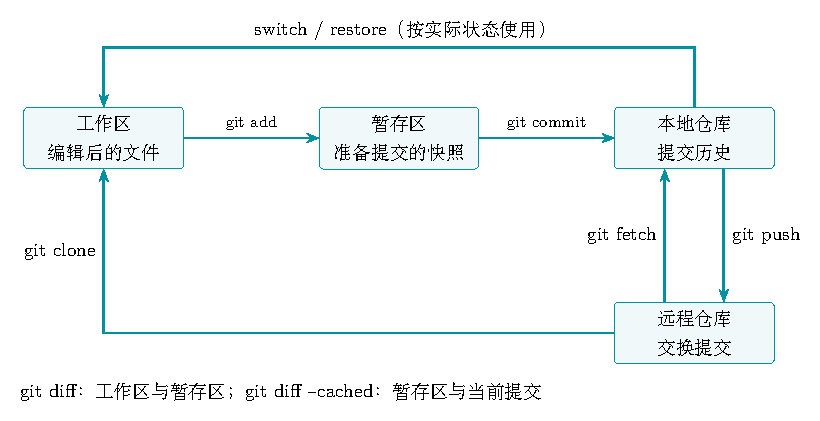
\includegraphics[width=0.9\textwidth]{git-workflow_revised.pdf}
\caption{Git 四个区域：箭头上的命令说明内容在哪两处之间流转}
\label{fig:git}
\end{figure}
顺着图里的箭头看，我们编辑好文件后，用 \texttt{git add 路径} 把当前版本放到暂存区。这里保存的是 add 时的版本，如果随后又改了同一个文件，还要重新 add。接下来用 \texttt{git commit -m '说明'} 把暂存内容记成一次本地提交，再用 \texttt{git push 远程 分支} 发给远程仓库，队友才能从那里获取。

如果不知道自己走到了哪一步，可以先看 \texttt{git status}。想看具体改动，\texttt{git diff} 比较工作区和暂存区，\texttt{git diff --cached} 比较暂存区和当前提交。这两个 diff 看的是不同位置，后面我们会用同一个文件对比一次。

\Needspace{8\baselineskip}
\begin{example}[只配置练习仓库的作者]
在新目录操作，名称可换成自己的：


\Needspace{11\baselineskip}
\begin{tbash}
mkdir git-config-lab
cd git-config-lab
git init --initial-branch=main
git config user.name 'Training Student'
git config user.email 'student@example.invalid'
git config --local --get user.name
git config --local --get user.email
\end{tbash}


执行后应该能读回刚设置的名字和邮箱。\texttt{git config [作用域] 键 值} 用来设置配置，\texttt{--get} 则读取它；这里不加全局作用域，只改当前练习仓库。如果以后想让自己的仓库通常都使用同一份身份，可以加 \texttt{--global} 设置当前用户的通用配置。还有一点别弄混：名字和邮箱是提交里的作者信息，不是 GitHub 登录认证，填了邮箱也不会自动获得推送权限。
\end{example}
\begin{exercise}\label{ex:v1-git-config}
新建独立仓库，设置并读回本地作者身份。解释 add 后再改文件为何可以同时出现“已暂存”和“未暂存”状态；通过一次实际修改核对。
\end{exercise}

\subsubsection{从修改到远程：不联网的完整实验}
\label{sec:git-local-demo}
概念看过了，我们来完整走一遍。项目放在本卷 \texttt{examples/git-workflow-demo/}，只有 \texttt{demo.sh} 和 \texttt{README.md}。这一次把“远程”也放在本地临时目录里，你不用先处理网站账号和网络认证，就能看清文件是怎样从自己的工作区走到队友那里去的。
\Needspace{8\baselineskip}
\begin{example}[两次提交与另一份克隆]
目录中唯一的核心脚本完整如下：

\lstinputlisting[language=bash,frame=single,numbers=left,breaklines=true]{examples/git-workflow-demo/demo.sh}

从本卷目录运行：


\Needspace{6\baselineskip}
\begin{tbash}
cd examples/git-workflow-demo
bash demo.sh
\end{tbash}


\texttt{git init --bare} 建立不含普通工作区的“远程”；\texttt{git clone 仓库 目录} 获取一份本地工作副本。脚本第一次写 camera 后 add、commit、push；第二次写 radar，先看工作区差异，再 add 看暂存差异，最后提交并推送。\texttt{-u} 记录上游，此后在同一分支可直接 push。

运行时先看看 WORKTREE DIFF，再看看 STAGED DIFF：里面都有新增的 radar，但它们出现在 add 前后两个阶段。最后 TEAMMATE CONTENT 应该是 camera、radar 两行，COMMIT COUNT 为 2。我们在 teammate 这份克隆里看到了两次提交，就说明它们确实已经进入远程，不只是留在 student 的本地仓库里。第一次克隆时提示空仓库，是因为我们刚刚创建的“远程”还没有内容；后面如果还有失败提示，就要按具体错误处理，不能都当成这条警告忽略掉。
\end{example}
\begin{exercise}\label{ex:v1-git-commits}
在脚本打印的 student 仓库中增加第三行并提交，先\textbf{不推送}。记录 student 和 remote 的提交数，再 push，最后在 teammate 中执行 \texttt{git pull --ff-only} 并检查第三行。解释为什么本地 commit 成功不代表队友已经收到。
\end{exercise}

\subsubsection{分支、合并与实际远程}
如果你正在写新功能，又不想把没写完的东西直接混进主线，我们就可以开一个分支（Branch）。它是指向某次提交的可移动名字，不是把整个项目永久复制一遍。等功能写完、差异也检查过了，再合并（Merge）回主线。分支 A 和分支 B 表示：我们联合！不过联合之前，还是先看清各自改了什么。
\Needspace{8\baselineskip}
\begin{example}[没有冲突的最小分支实验]
在刚才的 student 仓库中执行；开始前 \texttt{git status --short} 应为空，不能把未完成修改顺手混入实验：


\Needspace{11\baselineskip}
\begin{tbash}
git switch -c feature-note
printf 'check timestamps\n' > review.txt
git add review.txt
git commit -m 'Add review note'
git switch main
git merge --ff-only feature-note
git log --oneline --graph -4
\end{tbash}


执行完再看 main，应该已经出现了新文件，日志里也能找到刚刚的提交。因为 main 没有另外前进，它可以直接沿着这条历史走到新位置，这就叫快进。\texttt{--ff-only} 只允许这种情况；如果两条分支各自有了新提交，它会拒绝，而不是自动帮我们解决冲突。你在旧教程里看到的 \texttt{checkout -b 名称} 也能创建并切换分支，这里我们使用职责更明确的 switch。
\end{example}
\begin{exercise}\label{ex:v1-git-branch}
在自己的练习仓库创建另一个分支，增加一个小文件并提交，切回 main，合并并查看图形日志。指出分支名、提交与工作文件的关系，最后保留记录，不操作真实远程。
\end{exercise}

换成服务器仓库时，\texttt{git remote -v} 查看地址，\texttt{git fetch 远程} 取回提交但不合并工作区，\texttt{git pull} 包含取回及整合步骤，\texttt{git push} 把本地分支的提交发出去。HTTPS 的访问令牌与 SSH 密钥是认证方式，按托管服务说明设置，不在教材、脚本或提交中写凭据。已有上游时使用简短命令；无上游时先核对远程名和当前分支，不假设都叫 origin/main。
\begin{note}
\texttt{git reset --hard} 会丢弃所覆盖路径的未提交修改；强制推送会改写远程历史，影响队友。本章不需要这些操作。合并冲突时先读 status 和冲突块，确认两边意图，编辑后 add、commit；想取消未完成合并，可先保存新增工作，再按实际状态使用 \texttt{git merge --abort}。未提交内容没有可靠的 Git 恢复保证。
\end{note}

\subsubsection{忽略构建产物}
工程编译几次后，目录里通常会多出构建产物和日志，我们不必把它们每次都交给队友。可以用 \texttt{.gitignore} 告诉 Git，哪些未跟踪文件可以忽略。不过已经跟踪过的文件，不会因为写进了这份名单就自动退出历史。

常用的模式有 \texttt{*.log}（匹配日志）、\texttt{/build/}（仓库根目录下的 build）和 \texttt{!路径}（取消忽略）。如果想忽略 build 里的大部分文件，又保留一个例外，就要留意：把父目录整个忽略以后，Git 不会再进去寻找例外。下面我们实际试一下。
\Needspace{8\baselineskip}
\begin{example}[保留 build 中的一个文件]
在练习仓库创建 \texttt{.gitignore}：
\begin{lstlisting}[language={},frame=single]
*.log
/build/*
!/build/keep.txt
\end{lstlisting}
然后验证：


\Needspace{8\baselineskip}
\begin{tbash}
mkdir -p build
touch run.log build/cache.tmp build/keep.txt
git status --short --untracked-files=all
git check-ignore -v run.log build/cache.tmp
\end{tbash}


status 应列出 .gitignore 与 build/keep.txt，不显示另两项。已跟踪文件若确实要停止跟踪，可用 \texttt{git rm --cached 路径} 后提交；这保留工作文件，\textbf{不会抹去旧提交里的内容或泄露过的凭据}。
\end{example}
\begin{exercise}\label{ex:v1-git-ignore}
为自己新建的日志与构建目录设置上述忽略与例外规则，实际核对 status。解释先写 /build/ 再取消忽略 keep.txt 为何通常不能达到目标。
\end{exercise}
\begin{conclusion}
Git 操作先问“我正在改哪个区域”：编辑改工作区，add 更新暂存快照，commit 建本地历史，push 交换提交。分支组织历史，忽略规则控制未跟踪文件。每次提交前看 status、diff 和 diff --cached，避免把旧产物或无关文件一起交给队友。
\end{conclusion}
官方命令与忽略规则可在 \url{https://git-scm.com/docs} 查；想观察分支关系可用 \href{https://learngitbranching.js.org/?locale=zh_CN}{Learn Git Branching 中文版}，网页动画辅助理解，不能代替本地文件验证。
